\documentclass{article}
\usepackage{amsmath}
\usepackage{amssymb}
\usepackage{graphicx}
\usepackage{listings}
\usepackage{color}

\definecolor{dkgreen}{rgb}{0,0.6,0}
\definecolor{gray}{rgb}{0.5,0.5,0.5}
\definecolor{mauve}{rgb}{0.58,0,0.82}
\graphicspath{ {./.} }

\lstset{frame=tb,
  language=C++,
  aboveskip=3mm,
  belowskip=3mm,
  showstringspaces=false,
  columns=flexible,
  basicstyle={\small\ttfamily},
  numbers=none,
  numberstyle=\tiny\color{gray},
  keywordstyle=\color{blue},
  commentstyle=\color{dkgreen},
  stringstyle=\color{mauve},
  breaklines=true,
  breakatwhitespace=true,
  tabsize=3
}

\begin{document}
\author{Paraschiv Tudor-Andrei Grupa A5}
\title{TopMusic(B)\\Documentație}
\maketitle
\newpage

\section{Introducere}
\hspace{4mm}Acest raport va prezenta detalii pentru realizarea proiectului "TopMusic(B)" în limbajul C/C++ cu cerințele specificate în pagina cursului.

	Aplicația este alcătuită din două componente: componenta client care permite introducerea unor comenzi folosind terminalul, și componenta server care primește comenzile și execută comenzi SQL. După verificarea și executarea comenzilor, rezultatul final va fi transmis spre client.

	În secțiunile următoare sunt prezentate detalii despre implementarea și arhitectura aplicației.
\section{Tehnologii utilizate}
\hspace{4mm}Pentru conexiunea dintre client și server, va fi utilizat modelul TCP concurent pentru a permite conectarea mai multor clienți la server. 

După acceptarea unui client, serverul va creea un thread separat pentru acesta, astfel servind un număr variabil de clienți simultan. Pentru stocarea și gestiunea datelor, aplicația folosește librăria SQLite 3 care creează legătura dintre server și baza de date.


\section{Arhitectură}
\hspace{4mm}Aplicația server și cea client folosesc o librărie comună "enums.h" pentru a identifica și executa comenzile definite. După realizarea conexiunii, serverul va creea un thread separat pentru client care va permite transmiterea și receptarea mesajelor. Odată ce o comandă a fost identificată, va fi executată funcția dedicată acelei comenzi pentru accesul sau scrierea în baza de date. La finalizarea operației, va fi transmis clientului un mesaj specific în funcție de succesul sau eșecul comenzii SQL.
	
Baza de date conține 6 tabele care conțin informații despre utilizatori, administratori, melodii, cereri pentru adăugarea melodiilor, comentarii și voturi. Pe lângă acestea, tabela $sqlite\_sequence$ conține cele mai mari valori din cheile primare pentru a le incrementa automat. În baza de date $topmusic.db$ din arhivă, sunt introduse câteva date pentru testarea aplicației. 

\pagebreak
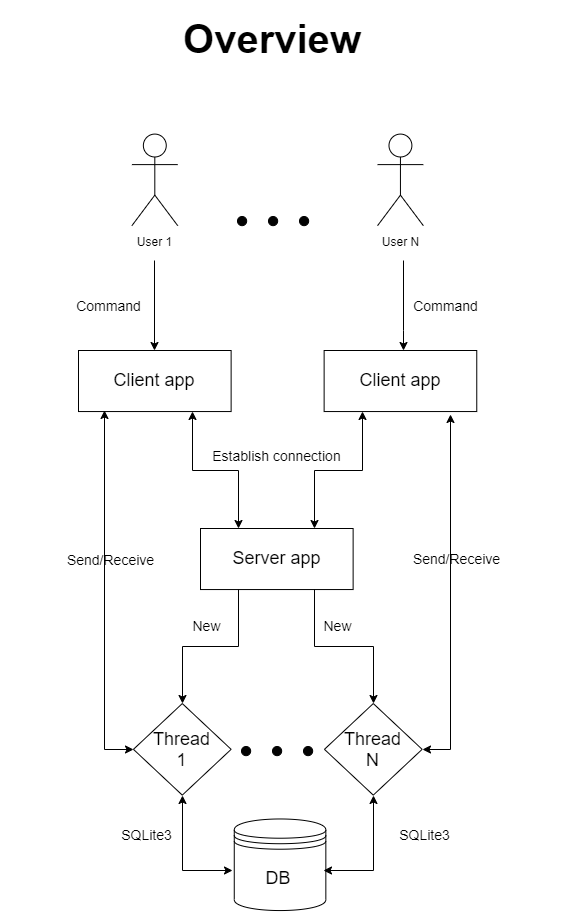
\includegraphics[width=\textwidth]{overview}

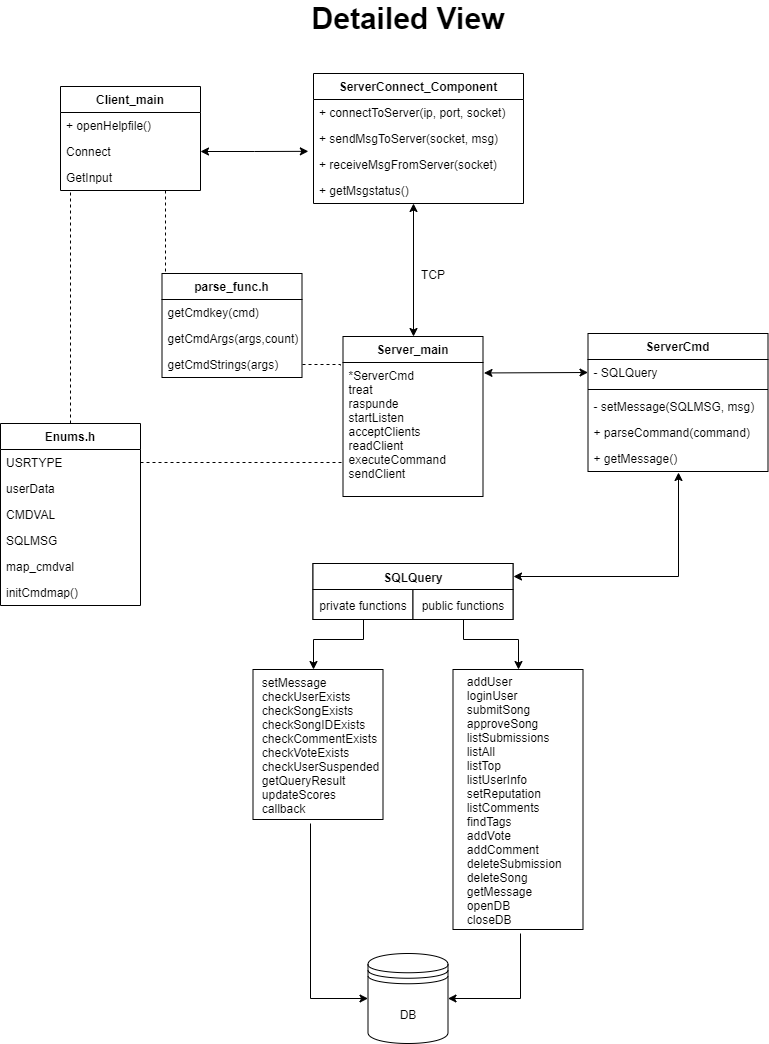
\includegraphics[width=\textwidth]{details}
\pagebreak

\pagebreak
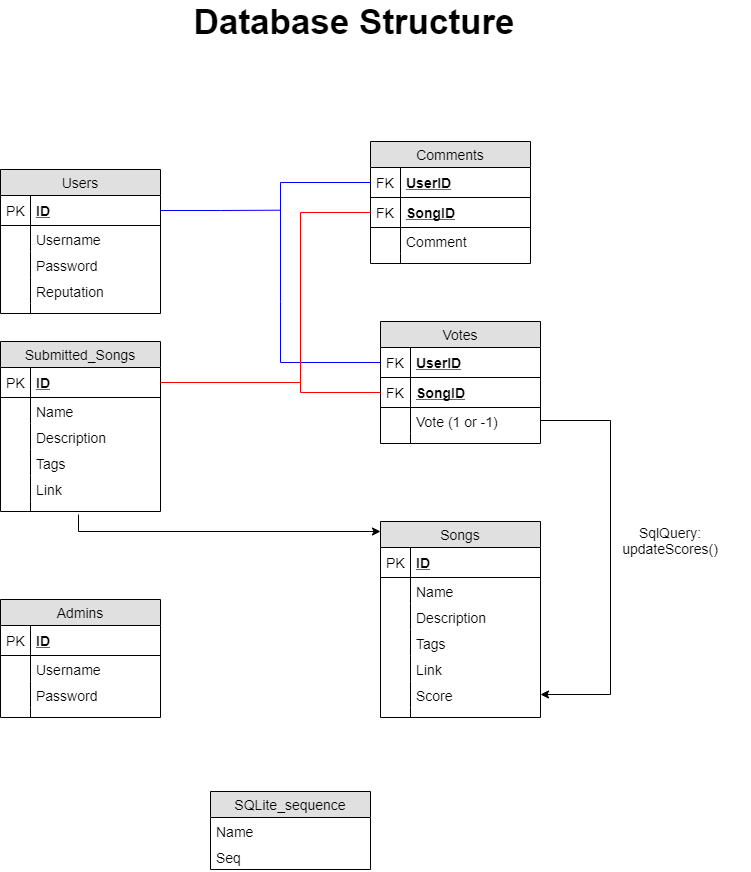
\includegraphics[width=\textwidth]{dbstruct}

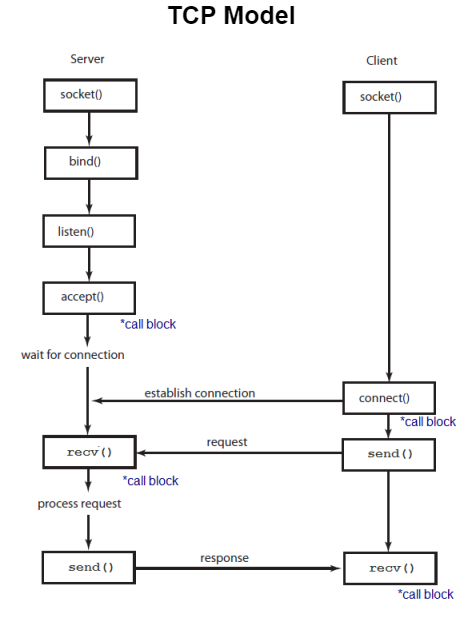
\includegraphics[width=\textwidth]{tcp}
\pagebreak


\section{Detalii de implementare}

\hspace{4mm} Clientul folosește clasa $ServerConnect\_Component$ pentru conexiunea și schimbul de mesaje cu serverul. Un mesaj conține un număr format din 3 cifre care reprezintă starea de succes/eșec a comenzii și un șir de caractere care descrie mesajul propriu-zis. Numarul din începutul mesajului nu este afișat pe ecran. 

Librăria $enums.h$ conține structurile de date folosite de client și server. Enumerarea $USRTYPE$ este folosită pentru marcarea sau identificarea user-ului ca admin sau utilizator normal. Structura $userData$ conține tipul, id-ul și două variabile pentru a determina dacă utilizatorul este conectat și logat. Enumerarea $SQLMSG$ conține valori pentru starea de succes sau eșec a unei comenzi. Enumerarea $CMDVAL$ conține valorile pentru toate comenzile definite, și este folosită împreună cu structura $map\_cmdval$ care atribuie unui șir de caractere o valoare din enumerarea comenzilor.

Librăria $parse\_func.h$ conține funcțiile pentru extragerea comenzilor și argumentelor specifice din mesajul transmis de client. Funcția $getCmdkey(command)$ extrage cheia comenzii și returnează o valoare din enumerarea $CMDVAL$ pentru a fi folosită într-un switch. $getCmdArgs(std vector, string args, count=0)$ extrage argumentele comenzii într-un vector iar $getCmdStrings(std vector, string args)$ extrage argumentele de tip string. Argumentele de tip string sunt delimitate de ghilimele și sunt folosite pentru introducerea datelor care conțin spații în baza de date. 
Exemplu:
\begin{lstlisting}
//command=submsong "Song Title" "Song description goes here" "tag1, tag2" "link.com"
switch(map_cmdval[getCmdkey(command)])
    {
				(...)
        case CMD_SUBMITSONG:
            if(user.LOGGEDIN==true){
                getCmdStrings(args, command.substr(8, command.size()));
                if(args.size() < 4 || !(args[0].size()>0 && args[1].size()>0 && args[2].size()>0 && args[3].size()>0)){
                    setMessage(SQL_ERRGENERIC, "Error: Invalid arguments -- Submit format: submsong \"title...\" \"description...\" 	\"tag1, tag2...\" \"link.com...\"\n");
                    return;
                } query->submitSong(args[0], args[1], args[2], args[3]);
               
            }
            else{
               setMessage(SQL_ERRGENERIC, "Error: You need to be logged in to execute this command\n"); return;}
		break;
				(...)
	}
 
\end{lstlisting}

În aplicația client, utilizatorul trebuie să introducă comanda $conn\ IP\ PORT$ pentru a se conecta la server. Odată conectat, poate înregistra un nou cont folosind comanda $reg\ username\ password$ sau se poate loga cu $login\ username\ password$. După logare, va fi determinat automat dacă contul este administrator sau utilizator normal, iar următoarele comenzi vor putea fi folosite: 
\begin{itemize}
\item $submsong\ "Title..."\ "Description..."\  "tag1, tag2"\  "link.com"$ - Trimite o cerere cu o melodie pentru a fi adăugată. Aceasta va fi verificată de administratori iar apoi aprobată sau ștearsă
\item $findtags\ tag1\ tag2\ ...\ tagN$ - Gasește melodiile care conțin tag-urile specificate
\item $vote\ ID\ up|down$ - Votează o melodie. Voturile "up" vor adăuga un punct la scor iar "down" vor scădea. Scorul este calculat și actualizat automat după fiecare vot. Utilizatorii cu valoarea 1 în câmpul $Reputation$ din baza de date nu pot vota.
\item $comment\ ID\ "Comment\ here..."$ - Adaugă un comentariu la o melodie
\item $showcomments\ ID$ - Afișează comentariile unei melodii
\item $info\ username$ - Afișează informații despre un utilizator
\item $list\ top|all$ - Afișează topul sau toate melodiile
\item $logout$ - Delogare
\end{itemize}

Administratorii pot folosi comenzile precedente dar și următoarele:
\begin{itemize}
\item $stopsv$ - Oprește serverul și deconectează toți utilizatorii conectați
\item $list\ subm$ - Afișează cererile cu melodiile trimise de utilizatori
\item $appvsong\ ID$ - Aprobă o cerere și adaugă melodia automat iar apoi o șterge din lista cererilor
\item $delsubm\ ID$ - Șterge o cerere
\item $delsong\ ID$ - Șterge o melodie
\item $setrep\ username\ 0|1$ - Modifică reputația unui utilizator. Utilizatorii cu valoarea 1 nu mai pot vota.
\end{itemize}

Comenzile următoare pot fi folosite oricând:
\begin{itemize}
\item $help$ - Afișează lista comenzilor împreună cu descrierea lor
\item $disconn$ - Deconectează clientul de la server.
\item $exit$ - Oprește aplicația client. Va fi trimis un mesaj final pentru ca serverul sa închidă socket-ul
\end{itemize}

\pagebreak
\textbf{Secvențe de cod:}
\begin{lstlisting}
//Exemplu de functie de verificare in baza de date
bool SQLQuery::checkVoteExists(std::string user_id, std::string song_id)
{
    std::string checkcommand = "SELECT USERID FROM Votes WHERE USERID =" + user_id + " and SONGID=" + song_id + ";";

    struct sqlite3_stmt *selectstmt;
    rc = sqlite3_prepare_v2(db, checkcommand.c_str(), -1, &selectstmt, NULL);
    
    auto selected = sqlite3_step(selectstmt);
    sqlite3_finalize(selectstmt);
    
    if(rc == SQLITE_OK)
    {
        if (selected == SQLITE_ROW)
                return true; 
        else 
                return false;
    }
    else
    {
        return false;
    }
}
\end{lstlisting}

\begin{lstlisting}
//Functia pentru suspendarea de la vot a unui utilizator
void SQLQuery::setReputation(std::string name, std::string rep_value)
{//set reputation for a user 0=neutral 1=vote suspended
    if(checkUserExists(USER, name)){
        std::string command = "UPDATE Users SET Reputation=" + rep_value + " WHERE username=\'" + name +"\';";
        int rc = sqlite3_exec(db, command.c_str(), callback, 0, &szErrMsg);
        if(rc != SQLITE_OK)
        {
            printf("SQLerror:%s\n", sqlite3_errmsg(db));
            setMessage(SQL_ERRGENERIC, "Error: Could not set reputation, check rep value (0 normal, 1 suspended)");
        }
        else
            setMessage(SQL_SETREPSUCCESS, "Changed user reputation"); 
    }
    else
        setMessage(SQL_ERRGENERIC, "Error: Could not find user");
}
\end{lstlisting}
\pagebreak
\begin{lstlisting}
//Functia pentru afisarea melodiilor din top
void SQLQuery::listTop()
{
    sqlite3_stmt *stmt;
    char command[] = "SELECT * FROM Songs ORDER BY Score DESC LIMIT 5;";
    
    int rc = sqlite3_prepare_v2(db, command, -1, &stmt, NULL);
    if(rc != SQLITE_OK)
    {
        printf("error: %s", sqlite3_errmsg(db));
        setMessage(SQL_ERRGENERIC, "Error: List failed");
    }
    else
    {
        char result[MSG_BUFSIZE];
        getQueryResult(stmt, result);
        setMessage(SQL_NULL, result);
    }
    sqlite3_finalize(stmt);
}
\end{lstlisting}
\begin{lstlisting}
//Functie pentru extragerea string-urilor din argumentele unei functii
void ServerCmd::getCmdStrings(std::vector<std::string> &vector, std::string args){
    if(args[0]==' ')
        args.erase(0,1);
    std::string temp;
    bool reading_chars = false;
    for(int i=0; i < args.size(); i++) {
        if((args[i]==' ' && args[i+1]=='\"') || (i==0 && args[i]=='\"')){
            if(i!=0)
                i++;
            reading_chars = true;
            temp = "";
            continue;
        }
        if(reading_chars){
            if(args[i]=='\"' && (args[i+1]==' ' || args[i+1] == '\0'))
            {
                reading_chars = false;
                vector.push_back(temp);
                continue;
            }
            temp+=args[i];
        }
    }
}
\end{lstlisting}
\pagebreak
\textbf{Alte detalii:}

Un cont de administrator poate fi înregistrat doar folosind comanda \linebreak $areg\ username\ password\ adminkey$, cheia admin fiind definită în $enums.h$\linebreak(valoarea prestabilită este "adkey12345").

Serverul poate fi executat cu un argument de tip int pentru a seta portul, altfel valoarea acestuia va fi 5005.

Lista comenzilor poate fi consultată și în fișierul $help.txt$ din arhivă. Fără acest fișier, aplicația client nu va putea afișa detaliile din comanda $help$.

\section{Concluzii}
\hspace{4mm} Aplicația client ar putea beneficia de mai multe funcționalități pe baza mesajelor de succes/eșec (interfață text sau grafică). 

Aplicația nu reține în baza de date parolele utilizatorilor într-un mod securizat. Aplicația client ar putea transforma orice parolă introdusă într-un hash MD5 sau PBKDF2, iar apoi hash-ul poate fi transmis spre server pentru a fi verificat în baza de date.

Pentru îmbunătățirea vitezei de transfer a datelor, modelul UDP este o opțiune mai buna față de cel TCP. În schimb, modelul UDP nu va garanta integritatea datelor.



\section{Bibliografie}
\subsection{Site-uri}
https://profs.info.uaic.ro/\textasciitilde computernetworks/
\linebreak
https://profs.info.uaic.ro/\textasciitilde bd/wiki/index.php/Pagina\_principală
\linebreak
https://www.overleaf.com/learn
\linebreak
https://stackoverflow.com/questions/tagged/c
\linebreak
https://stackoverflow.com/questions/tagged/c++
\linebreak
https://www.sqlite.org/docs.html
\linebreak
https://en.cppreference.com/w/cpp
\linebreak
https://en.cppreference.com/w/c
\linebreak
https://sourcemaking.com/
\linebreak

\subsection{Cărți}
C/C++ Programmer's Bible by Kris Jamsa, Lars Klander

\end{document}